\newcolumntype{L}{>{\centering\arraybackslash}m{4.5cm}}

\chapter{Evaluation}
\label{cha:evaluation}
 
In this chapter we evaluate and analyze our implementations of the Stop Detections, Clusterings and Graph processing. 
 
\section{Location data characteristics for Berlin area}

We have worked with movement triggered data from mobile devices are spanned across Germany. Plotting the data gave us the picture shown in \autoref{fig:ger_points}.

\begin{figure}[!ht]
	\centering
	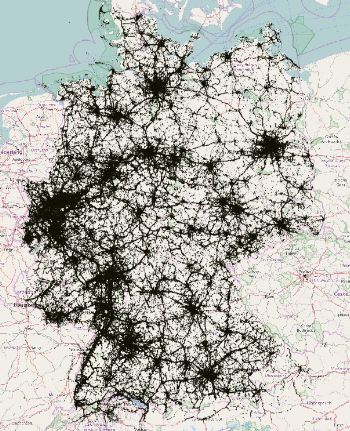
\includegraphics[width=0.5\textwidth]{images/points_germany.png}\\
	\caption{Visualisation of data points location in the geographical map of Germany}
	\label{fig:ger_points}
\end{figure}
\FloatBarrier

It turns out that most of the detected movements from one point to another are mostly gathered on the highways and inside the cities. Since our given points are updated on movement this is reasonable.  

\begin{figure}[!ht]
	\centering
	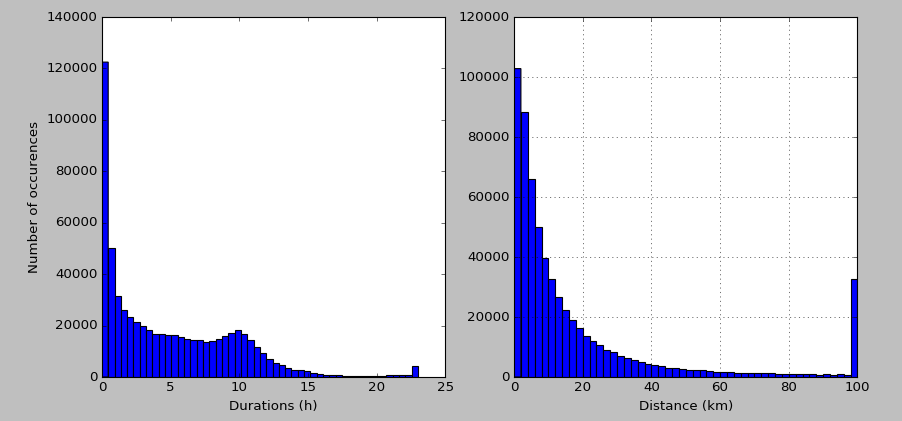
\includegraphics[width=0.9\textwidth]{images/germany_stats.png}\\
	\caption{Histograms of duration and distances between consecutive points under and cumulatively over 100 km for the area of Germany}
	\label{fig:ger_stats}
\end{figure}
\FloatBarrier

The given data batch has been gathered in the interval of 24h starting from 3am in the morning. It consists of over 675000 data points, belonging to 47300 unique mobile devices. \autoref{fig:ger_stats} shows, that for unique mobile devices, the duration between consecutive points in time are most frequent within 30 minutes and most of the data is in the interval of 1-10 h. Regarding distances, consecutive points are most frequent below 2 km and most data is in the interval 0-10 km. Big chunk of distances is also over 100 km. 

\begin{figure}[!ht]
	\centering
	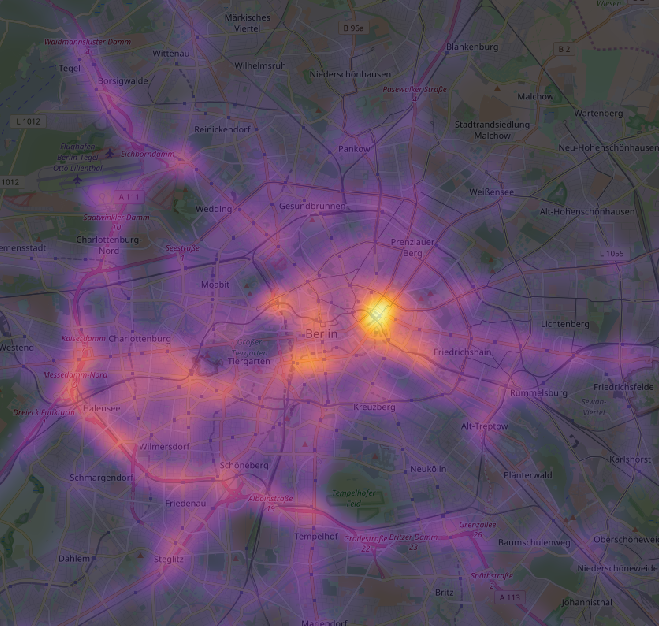
\includegraphics[width=0.9\textwidth]{images/points_berlin_heatmap.png}\\
	\caption{Heatmap of data point densities within the area of Berlin}
	\label{fig:ber_heat}
\end{figure}
\FloatBarrier
\autoref{fig:ber_heat} shows the heatmap of data points for Berlin area. We can see that most of the movements detected are on major train/tram/metro stations, highways and major living areas. 

\subsection{Data analysis}
\label{cha:dataanaly}

Data analysis had shown, that the users at least once visiting Berlin, had in average 17 points gathered in the period of 24h, harmonic mean of 4 points and maximum 100 points.

\begin{figure}[!ht]
	\centering
	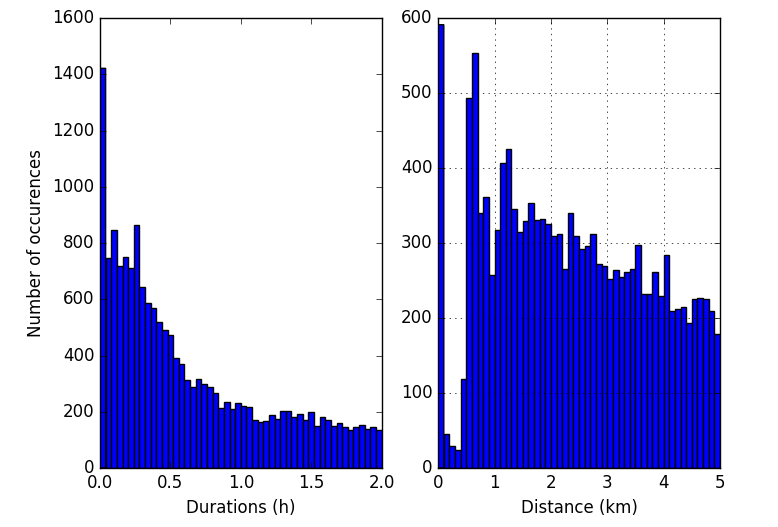
\includegraphics[width=0.6\textwidth]{images/berlin_stats_intro.png}\\
	\caption{Histograms of durations and distances between consecutive points under 5 km and under durations of 2h for the area of Berlin}
	\label{fig:ber_stats}
\end{figure}
\FloatBarrier

Furthermore, majority of duration between points are within intervals of 30 minutes. For distances between points, there are significant "jumps" at 500-1000m and 1100-1500m, which might mean that at these intervals, continuous points been gathered, and distances over that values might be discontinuous (ref. \autoref{fig:movement_update} ). It is due to the fact that these distance intervals are most frequent and that might suggest that this is an average "update" distance for the moving mobile devices. Less frequent values might suggest that updates were obtained with lower accuracy (e.g. by presence inside the building, metro line or simply mobile device lag in obtaining its location) and are result of discontinuity between consecutive updates.

\begin{figure}[!ht]
	\centering
	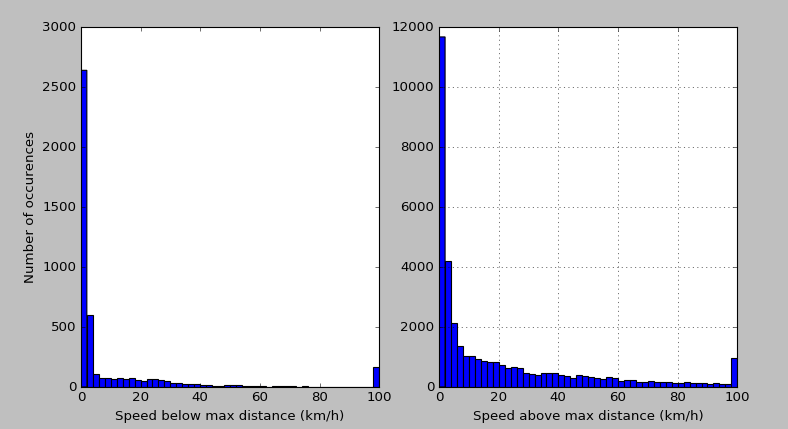
\includegraphics[width=0.6\textwidth]{images/berlin_speeds_distances.png}\\
	\caption{Histogram of speed between points with corresponding distance above or below 1.5 km}
	\label{fig:ber_sp_dis}
\end{figure}
\FloatBarrier

\autoref{fig:ber_sp_dis} shows that considering the registered distances within range of 1500m, the wast majority of points are between 0-2 km/h, and also significant interval at 2-6 km/h. The rest of the values is sparse distributed in interval 6-100+ km/h. In case of registered point above range of 1500m, we observe that indeed most frequent occurrence is at interval of 0-4 km/h, however most are sparse distributed above 4 km/h, with most points being in interval of 4-20 km/h. 

\section{Pre-filtering of anomalies}
\label{cha:prefilter}
\autoref{fig:ber_stats} shows that there is a fraction of points which duration or distance rapidly changed, thus resulting in very high speeds between the points. Points having speeds above 300 km/h and distances above 100km can be considered as flights, however the ones below 100km are anomalies. \autoref{fig:anom1} shows that number of flights in Germany has not been significant (around 100) compared to number of speed anomalies (over 25000).

Furthermore, due to the methodology of obtaining points (movement triggered), there are some minimum distances and durations at which points can be collected, and values not matching stop or travel expectation according to gathered statistics, have to be filtered and considered as duplicates. 

\begin{figure}[!ht]
	\centering
	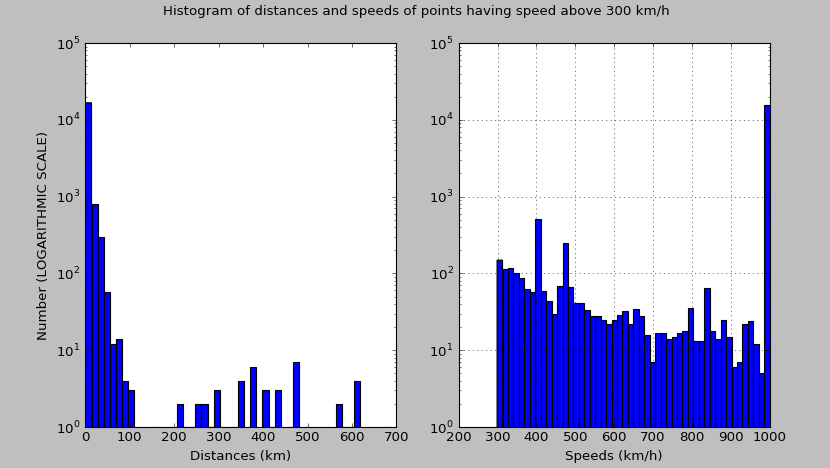
\includegraphics[width=0.6\textwidth]{images/anom1.png}\\
	\caption{ Speeds and distances histogram of points having speeds above certain threshold }
	\label{fig:anom1}
\end{figure}
\FloatBarrier

Thus, the following predicates for filtered values have been set:
\begin{description}
	\item[Jumps] Points with speed over 83 m/s [300 km/h] and at the same time distance below 100 km/h
	\item[Duplicates] Points with distance below 100m and at the same time duration below 100s
\end{description}

\section{Stop detection algorithm}
\label{cha:eval_stopdetc}

\subsection{Mobility Index approach}

Mobility Index analysis is performed in order to detect single movements or series of movements to be classified as stop or slow movement over the restricted area. 

By the nature of mobility index, more values in the window, higher the mobility index is. Thus, if only one value is in the window, one can apply "stop duration" threshold, however if windows contains more values, we require higher threshold to be able to fit sum of inverses of the movements. 

As an example, having window of 20 minutes and threshold of 1/(10 minutes), if we fit into window single point with duration of 15 minutes, this value will be classified as a stop. However, if we obtain 2 values, 5 and 10 minutes respectively (1/5 + 1/10), our threshold requires to be higher in order to include slow movements in the window and classify this 2 values as stop in restricted area.

\begin{figure}[!ht]
	\centering
	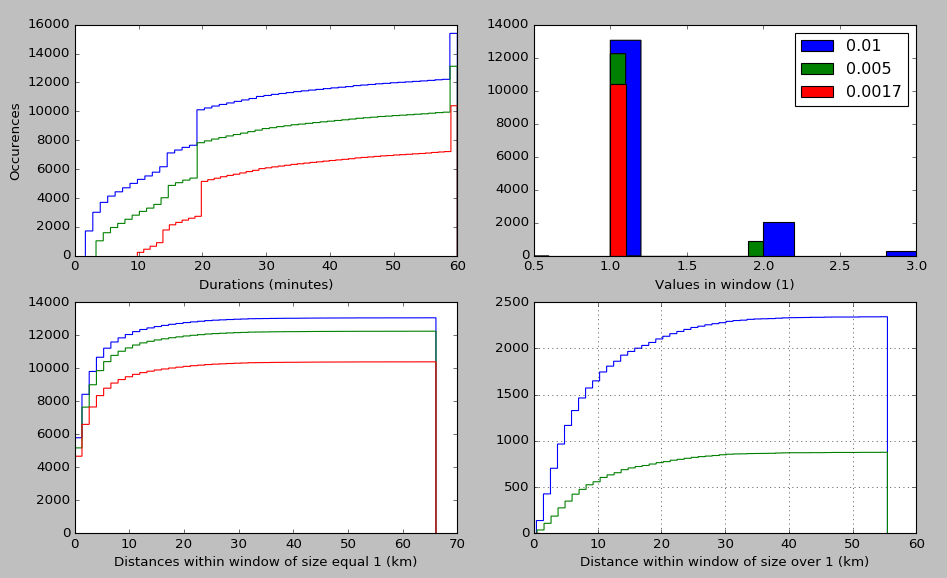
\includegraphics[width=0.95\textwidth]{images/mob_index_analy1.png}\\
	\caption{ Analysis of detected stops for varying MobilityIndexThreshold for time window of 20 minutes. Cumulative distribution of inverted mobility index (top left). Histogram of window sizes (top right). Cumulative distributions of total distances between points in the window of size 1 (bottom left) and above 1 (bottom right). }
	\label{fig:mob_index_analy1}
\end{figure}
\FloatBarrier

\autoref{fig:mob_index_analy1} shows the analysis of the stops detected using mobility index, using sliding time window approach.

Cumulative distribution of inverted mobility index (top left) shows that for window of 20 minutes, increasing MobilityIndexThreshold from 0.0017 (1/10 minutes) to 0.01 (1/2minutes), sum of inversions of durations (MobilityIndex) for points within the window, increases total number of stops from 10000 to 15000, where the increase (5000 points) is caused by points in the range 2-10 minutes, which is expected result increasing the threshold. The rapid jump at 20 minutes is caused by the fact that at that threshold some inverted mobility indexes were result of summing window of more then one value. 

Histogram of sizes of the window (number of points within a 20 minutes window - top right) shows, that with parameter 0.0017, all the points are contained within the windows having size of 1 point. Increasing the threshold to 0.005 (1/4 minutes), it resulted in 95 percent of points being in windows of size 1 and 5 percent in windows of size 2 (2 points in the window - restricted area of stop). Doubling the threshold to 0.01 resulted in 75 percent being in single value window, and 25 percent in over 2 points per window. 

The graphs in the bottom of \autoref{fig:mob_index_analy1} show what are the distances covered in the windows having 1 or more points. It occurs, that in case of 1 point in the window (which means that this point is a stop), distances between points range from 0 to 60km, and this is expected. However, in case of 2 or more points per window (thus stops within a restricted area bound by points), it occurs that only small fraction of values has total distance covered less then 2km, and major fraction of points represent long distance covered. 

The above analysis shows, that mobility index cannot be effectively used to detect group of points which might be considered as a stop and only very small fraction of windows having more points then 1 is considered as a stop within a small restricted area. The rest is spanned across bigger distances. Thus, small values of mobility index window and threshold might start detecting trips over longer distance as a stop and providing erroneous results. 
  
\begin{figure}[!ht]
	\centering
	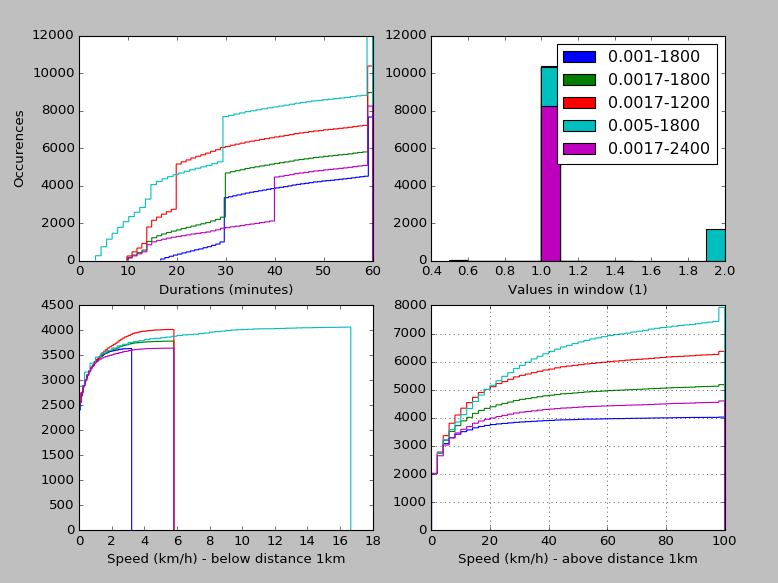
\includegraphics[width=0.95\textwidth]{images/mob_index_analy2.png}\\
	\caption{ Analysis of detected stops for varying MobilityIndexThreshold-MobilityIndexWindow(seconds), correspondingly as in the label of measurement. Cumulative distribution of duration for detected stops (top left). Histogram of window sizes (top right). Cumulative distributions of speed between point for distance below 1km (bottom left) and above 1km (bottom right). }
	\label{fig:mob_index_analy2}
\end{figure}
\FloatBarrier 
 
\autoref{fig:mob_index_analy2} shows the analysis of the stops detected using mobility index threshold, using sliding time window approach, however in this case it is used to identify mobility of a user considering only last recorded point in the window to decide if the movement can be a stop considering its past mobility.

This approach tries to tackle the problem discussed in \autoref{cha:stopdet_bh}, where it has been said that over longer distances e.g. 2-10 km between recorded points, detection using speed is difficult since stop for a short time and movement with high speed will produce very high average speed in that time period. 

\autoref{fig:mob_index_analy2} gives cumulative histograms considering different pair of parameters (MobilityIndexThreshold-MobilityIndexWindow) considered in producing stop locations. Cumulative distribution of duration at detected stops (top left) shows that considering the same MobilityIndexThreshold (0.0017-1200s, 0.0017-1800s, 0.0017-2400s) and increasing MobilityIndexWindow, causes less stops to be detected and higher average duration between points detected. Considering the same MobilityIndexWindow (0.001-1800s, 0.0017-1800s, 0.005-1800s) and increasing MobilityIndexThreshold, number of stops increases, and this increase is bound only to values below MobilityIndexWindow threshold. High MobilityIndexThreshold produces more stops with shorter duration of stop. 

Cumulative distribution of speed for detected points show that algorithm with all tested parameters has been able to identify correctly stops over distance less then 1km and with very small speeds (long stay duration at the point). However, MobilityIndexThreshold or decreasing MobilityIndexWindow cause that average speed of detected points had higher speed over distances > 1km and these were not able to filter trips over long distances correctly. For thresholds 0.001-1800s, 0.0017-1800s and 0.0017-2400s higher speeds are being filtered and only longer stays are left, and the difference between performance of these parameters is a trade-off between an accuracy and number of detected stops. 

Histogram of values in the window (top right) also confirms, that for 0.001-1800s, 0.0017-1800s and 0.0017-2400s thresholds, detected stops had window of 1 value, thus none of the windows having 2 or more values were not qualified for being a stop and thus being filtered out as high mobility trip. This behavior of algorithm allows to identify stays with simple duration threshold and at the same time filter out all multi-point trips using mobility index window. 

\subsection{Human Mobility approach for long/short distances}

Speed/Distance analysis is performed in order to detect single movements as stop or slow movement. If the average speed between the points is below the certain threshold, it is assumed to be a stop. 
 
\begin{figure}[!ht]
	\centering
	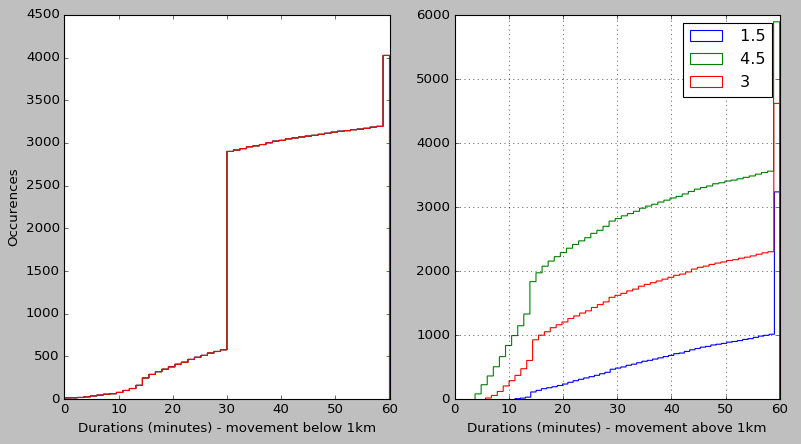
\includegraphics[width=0.95\textwidth]{images/speed_dist_analy1.png}\\
	\caption{Speed/Distance detection with StopCertaintyMaxDistance, StopCertaintyMaxSpeed and TravelCertaintyMinSpeed thresholds. Cumulative distribution of duration for detected stops below and above distance StopCertaintyMaxDistance of 1km for different  TravelCertaintyMinSpeed thresholds.}
	\label{fig:speed_dist_analy1}
\end{figure}
\FloatBarrier 

\autoref{fig:speed_dist_analy1} shows analysis of detected stops having TravelCertaintyMinSpeed varying and StopCertaintyMaxSpeed fixed. Increasing the speed threshold for points above 1km, we observe that number of points in interval 15 to 60+ minutes stays fixed for all parameters, however increasing threshold increases number of stops detected in interval 5-15 minutes diracticaly. It means, that with these thresholds, much more movements which has very low duration over the distance are classified as a stop and identification might be erroneous to mislead long distance trip with a stop. 

Furthermore, having TravelCertaintyMinSpeed threshold of 1.5 m/s, we can see that speed threshold correctly identifies the stops, however the number of detected stops in the movements above 1km compared to mobility index approach is low (\autoref{fig:mob_index_analy2}).

On the other hand, for distances below 1km, speed detection has not only been able to identify longer stays at location, but also a short distance, very slow movements over the area, successfully. 

\section{Stop location clustering}

This section describes how we evaluated our DBSCAN algorithm and the choice of the \textit{epsilon}, and \textit{minimum points per cluster} parameter.

\subsection{DBSCAN}

 Running the DBSCAN with different parameters resulted in different cluster sizes and number of clusters. We focused on the target area of greater Berlin and surrounding towns. Plotting histograms and visualizing the result on a QGIS \cite{qis}  map helped us in our choice of parameters. Since we used the dense target area of inner Berlin the parameter choice was easier than for example targeting whole of Germany or a larger area. However, we saw that small tweaks of the parameters had big impacts of the resulting cluster sizes and number of clusters. Below we evaluate the two parameters

\subsection{Evaluation of \textit{eps}}

The \textit{eps} parameter (epsilon, radius of the cluster) was initially chosen by looking at the graininess (accuracy) of our given data set - points only occur about each \textbf{110 meter} (longitude and latitude with five decimals accuracy, approximated to meters) therefore 110 meter is called the \textit{minimum distance} between two points.  

We took Alexanderplatz in Berlin as an example cluster (a popular train stop area in Berlin). We interpret one cluster as being one stop point of interest, therefor for this zoom level we expect Alexanderplatz to be represented as one cluster. 

As noted previously, DBSCAN is very sensitive to the choice of its parameters. In the figure \ref{fig:0.001_5_gray} we run DBSCAN with \textit{minimum distance}  and \textit{minPts} = 5, which causes expected looking clusters of popular stop areas. When choosing a greater \textit{eps} of 220 meters we instantly get huge clusters which correspond to an abnormal amount of expected stop areas, seen in figure \ref{fig:002_5_gray}. 

\begin{figure}[!ht]
	\centering
	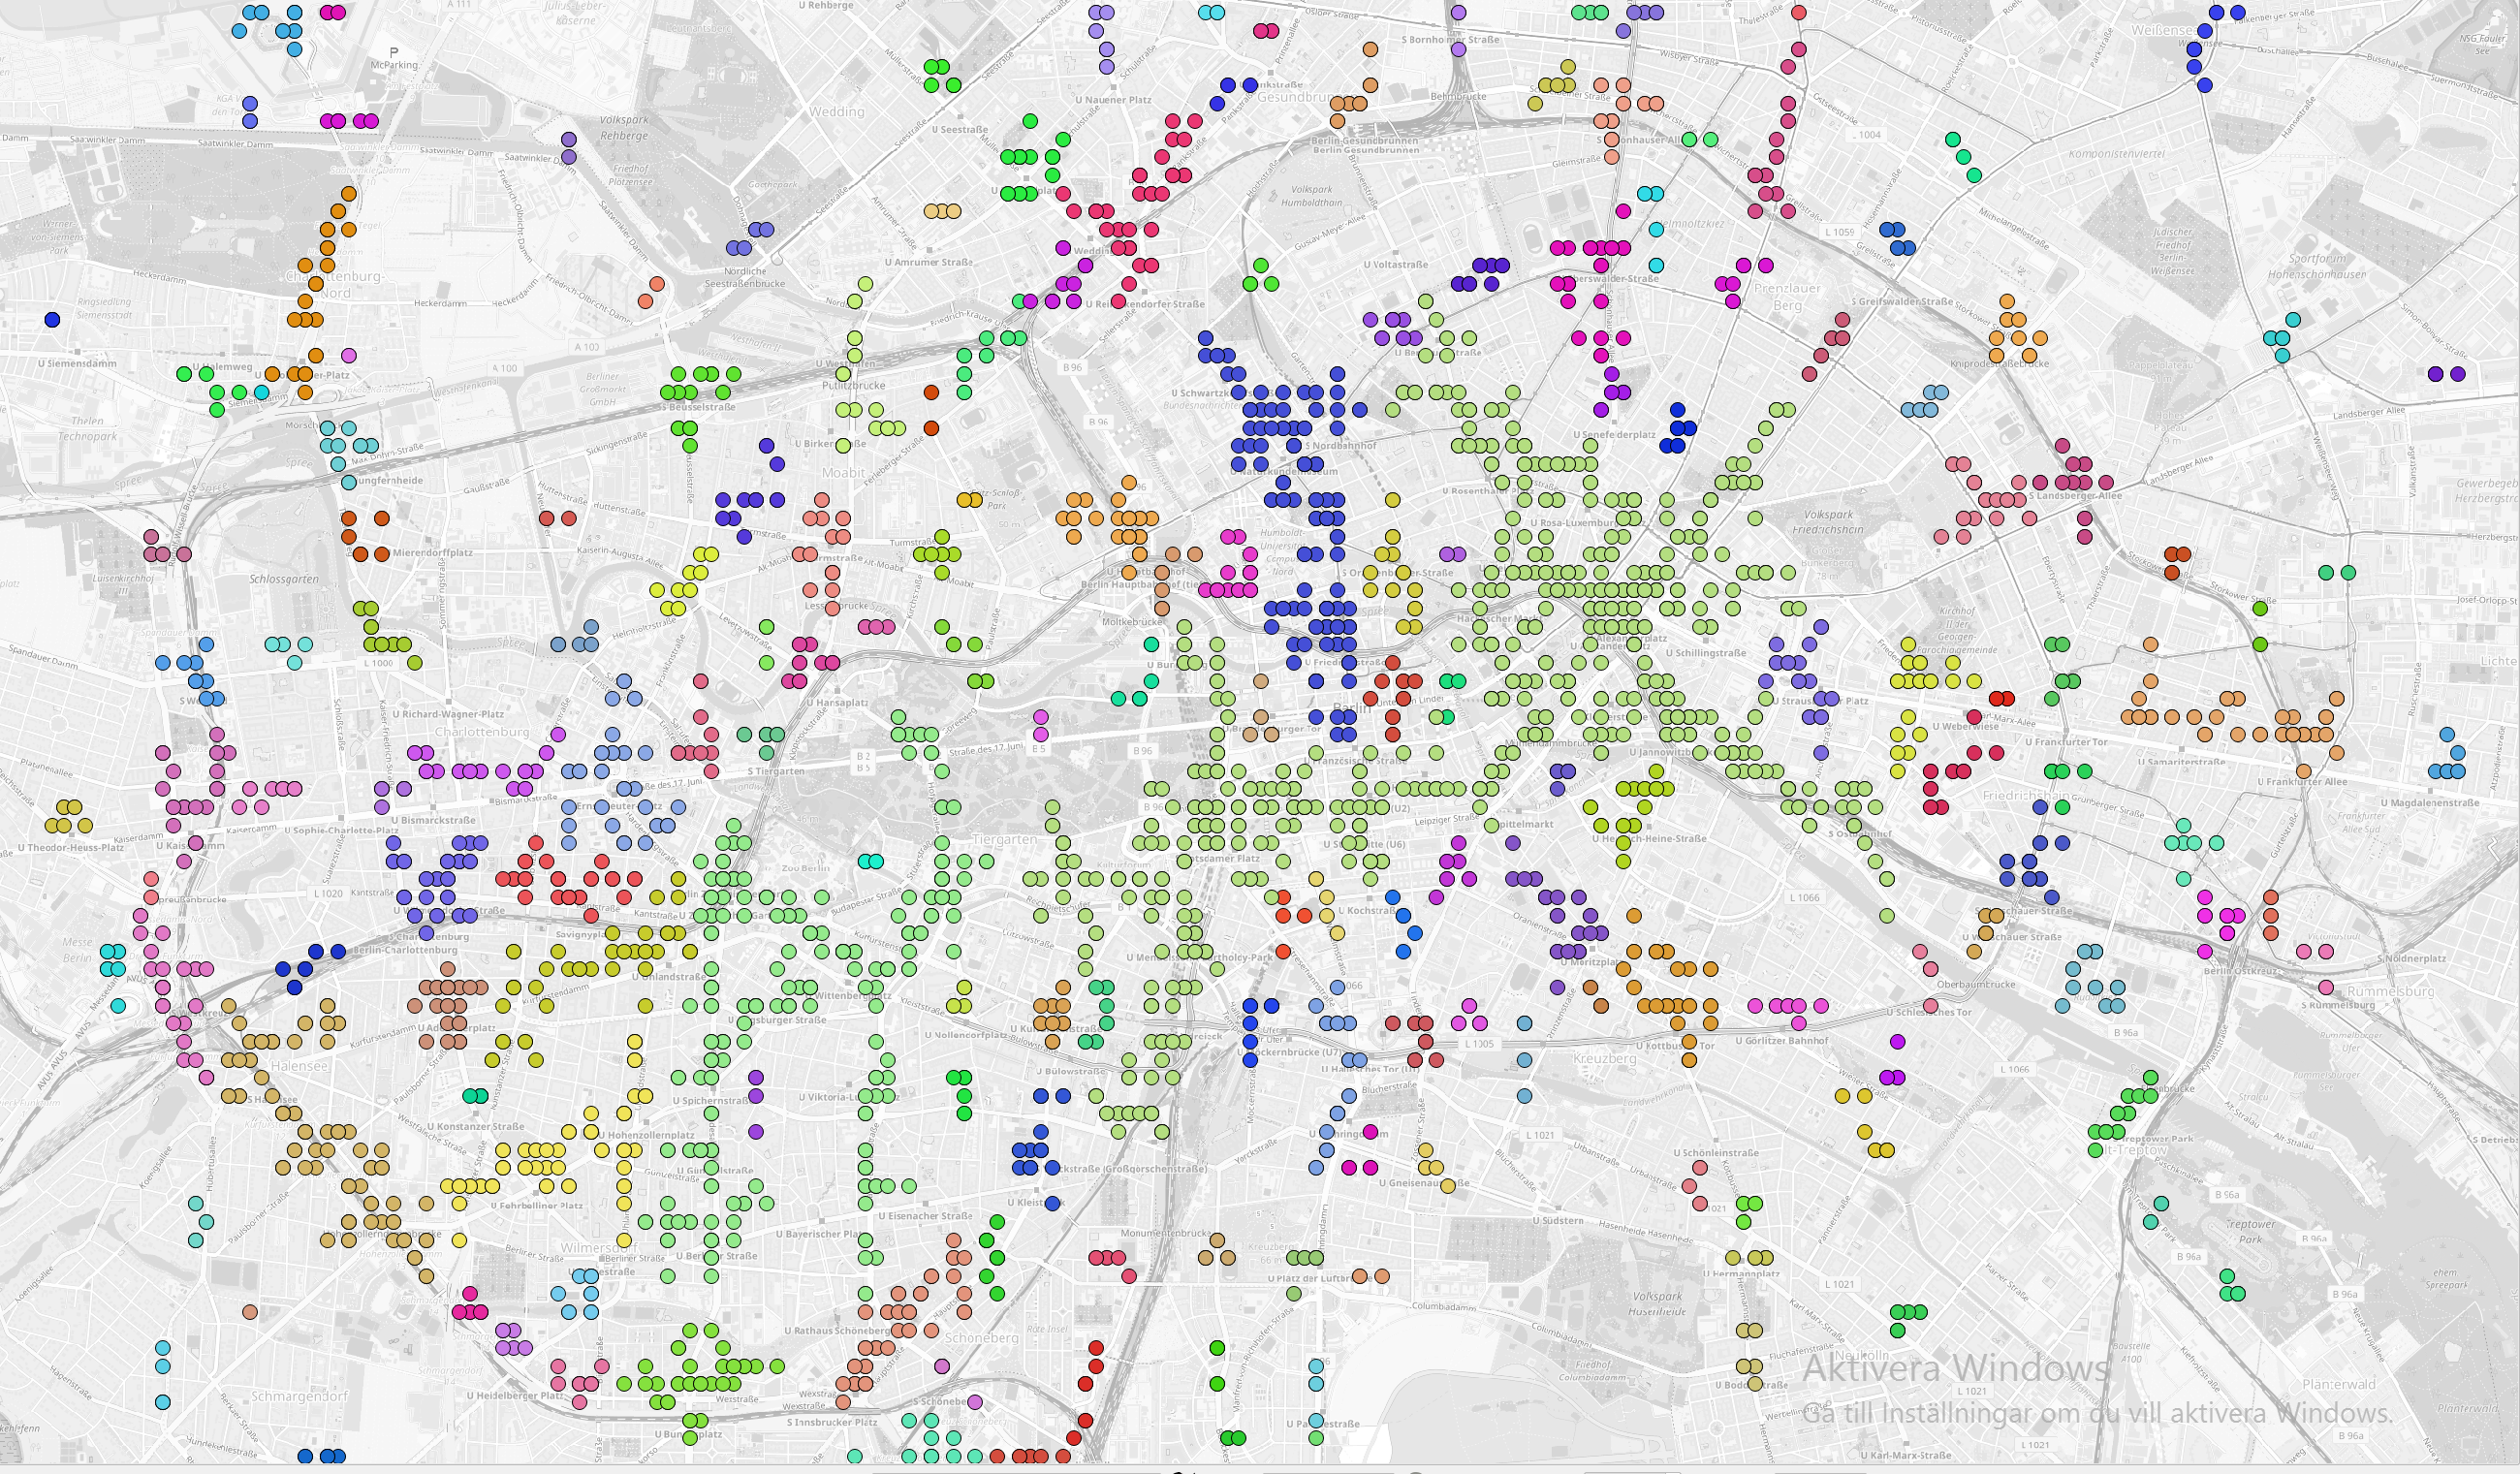
\includegraphics[width=0.8\textwidth]{images/0,002_5_gray.png}\\
	\caption{ Example of a clusters with bad parameters, here \textit{epsilon} = 220 meter is too large, \textit{minPts} = 5. "Alexanderplatz" (light green) has 748 data points in it and stretches over the whole centre (Mitte) of Berlin. }
	\label{fig:002_5_gray}
\end{figure}
\begin{figure}[!ht]
	\centering
	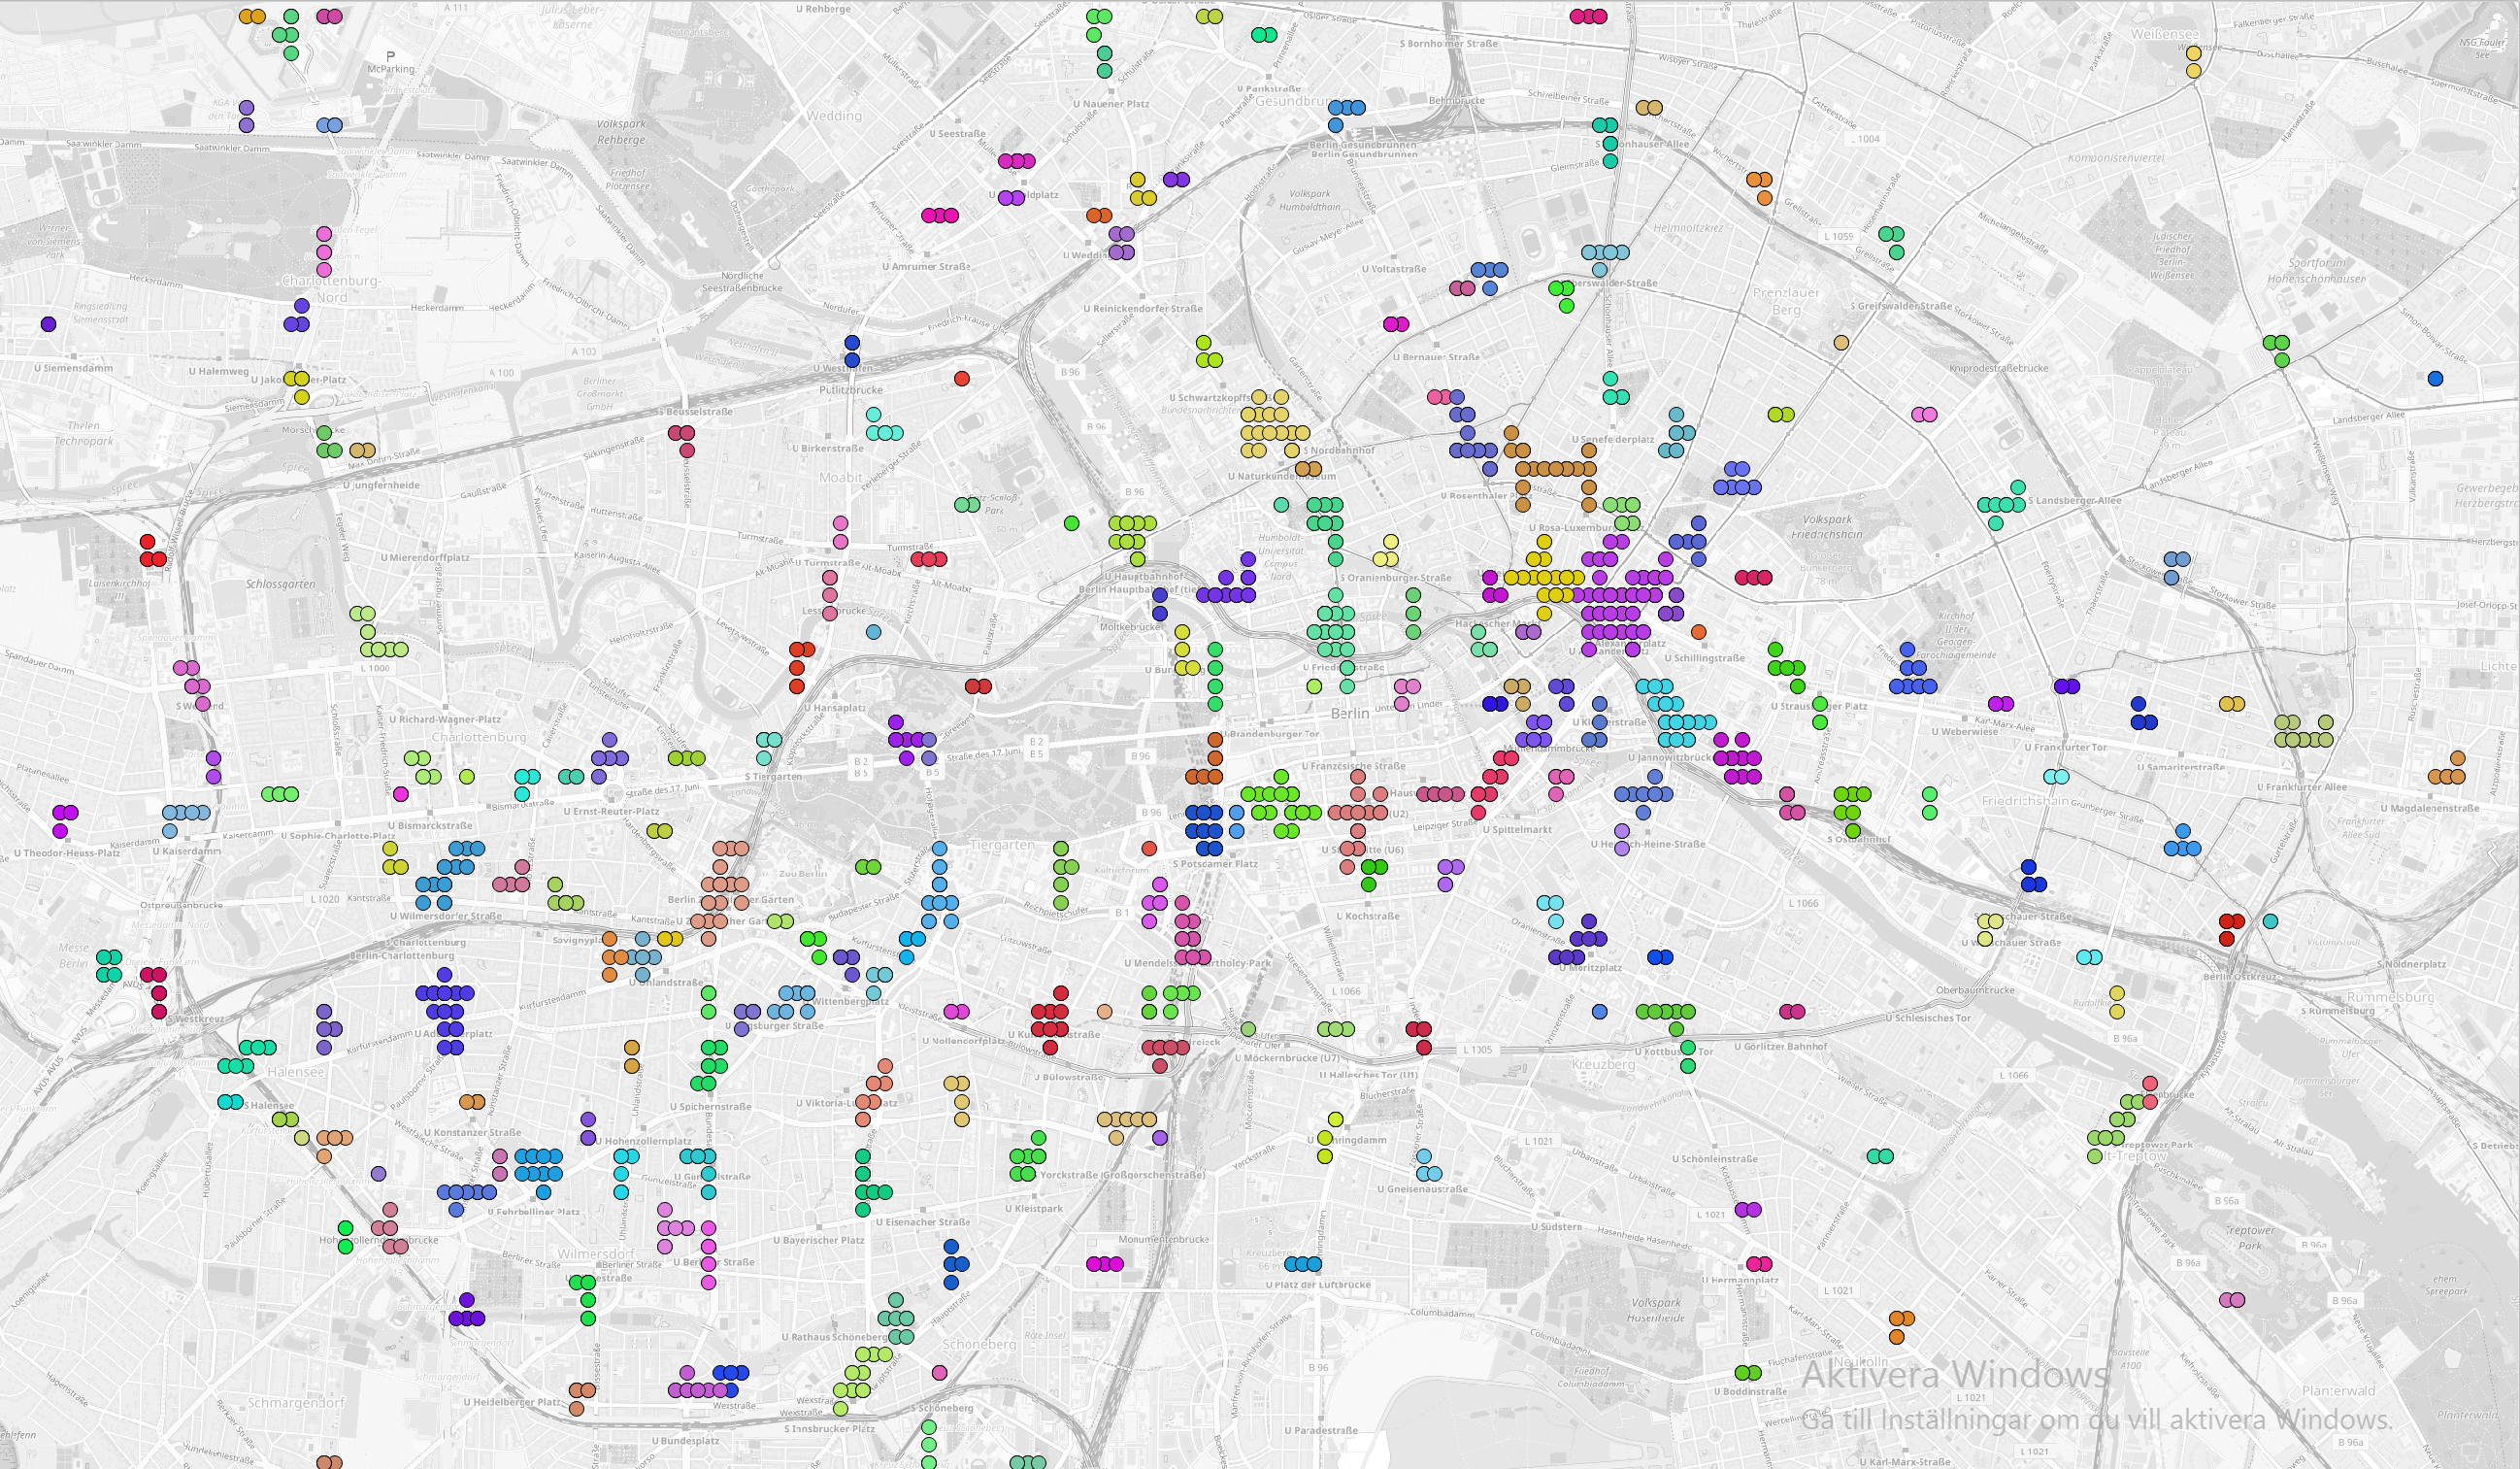
\includegraphics[width=0.8\textwidth]{images/0,001_5_gray.png}\\
	\caption{ Clusters with good parameters \textit{epsilon} = 110 meter, \textit{minPts} = 5. Alexanderplatz (pink) has 85 data points in it.  }
	\label{fig:0.001_5_gray}
\end{figure}
We concluded on the \textit{eps} parameter of 110 meters, the \textit{minimum distance}, since this gave us satisfying looking clusters for inner Berlin, whilst higher value of the parameter resulted in clusters being unnaturally large and \textit{eps} below the \textit{accuracy distance} resulted in only single-point clusters (points are stacked at the same location). 

\subsection{Evaluation of \textit{minPts}}

So far we have not discussed the \textit{minPts} parameter, minimum points per cluster. The parameter does not determine the size of the clusters but how many of them that has to be in one for it to be recognized as a cluster - which results in the number of clusters we get. Lower \textit{minPts} result in more found clusters, while higher result in less found clusters. The choice of \textit{minPts} was set by running DBSCAN multiple times with different values of the parameter and plotting them in histograms and on the map. We used the determined \textit{eps} of . 
\begin{figure}[!ht]
	\centering
	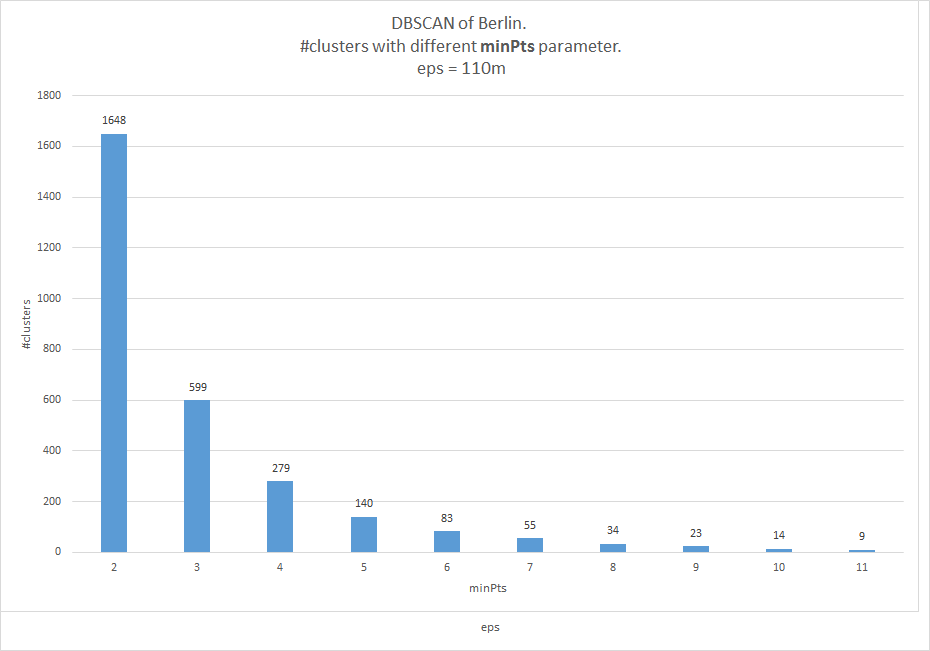
\includegraphics[width=0.8\textwidth]{images/histogram_minPts}\\
	\caption{ Histogram of number of clusters found from DBSCAN with different minPts. Higher \textit{minPts} captures significant fewer clusters . }
	\label{fig:histogram_minPts}
\end{figure}
In Berlin there are currently 173 U-bahn stops \cite{sbahn}. We would expect each stop to be represented as a stop point if our stop detection algorithm works well enough and we have enough data points. Since U-bahn stations usually are in areas of interest we could approximate the number of sought after clusters to a round this number. A number of detected stops between 100 and 200 hundred seems reasonable. As seen in the histogram in figure \ref{fig:histogram_minPts} setting \textit{minPts} to 5 gives us a cluster size of 140. Plotted on the map of our area, figure \ref{fig:0.001_5_gray}, gave us good looking result for inner Berlin. 


\subsection{Extending DBSCAN with areas}
 Our approach with using the same two fixed parameters, \textit{eps} and \textit{minPts}, worked well for inner Berlin. However, when zooming out and running our algorithm on a less dense area, such as greater Berlin, we encounter problem with few detected clusters. To fix this and detect more clusters we needed to increase the \textit{eps} parameter, however this caused problems with \textbf{huge} clusters in central Berlin as seen in figure \ref{fig:huge_cluster}.
\begin{figure}[!ht]
	\centering
	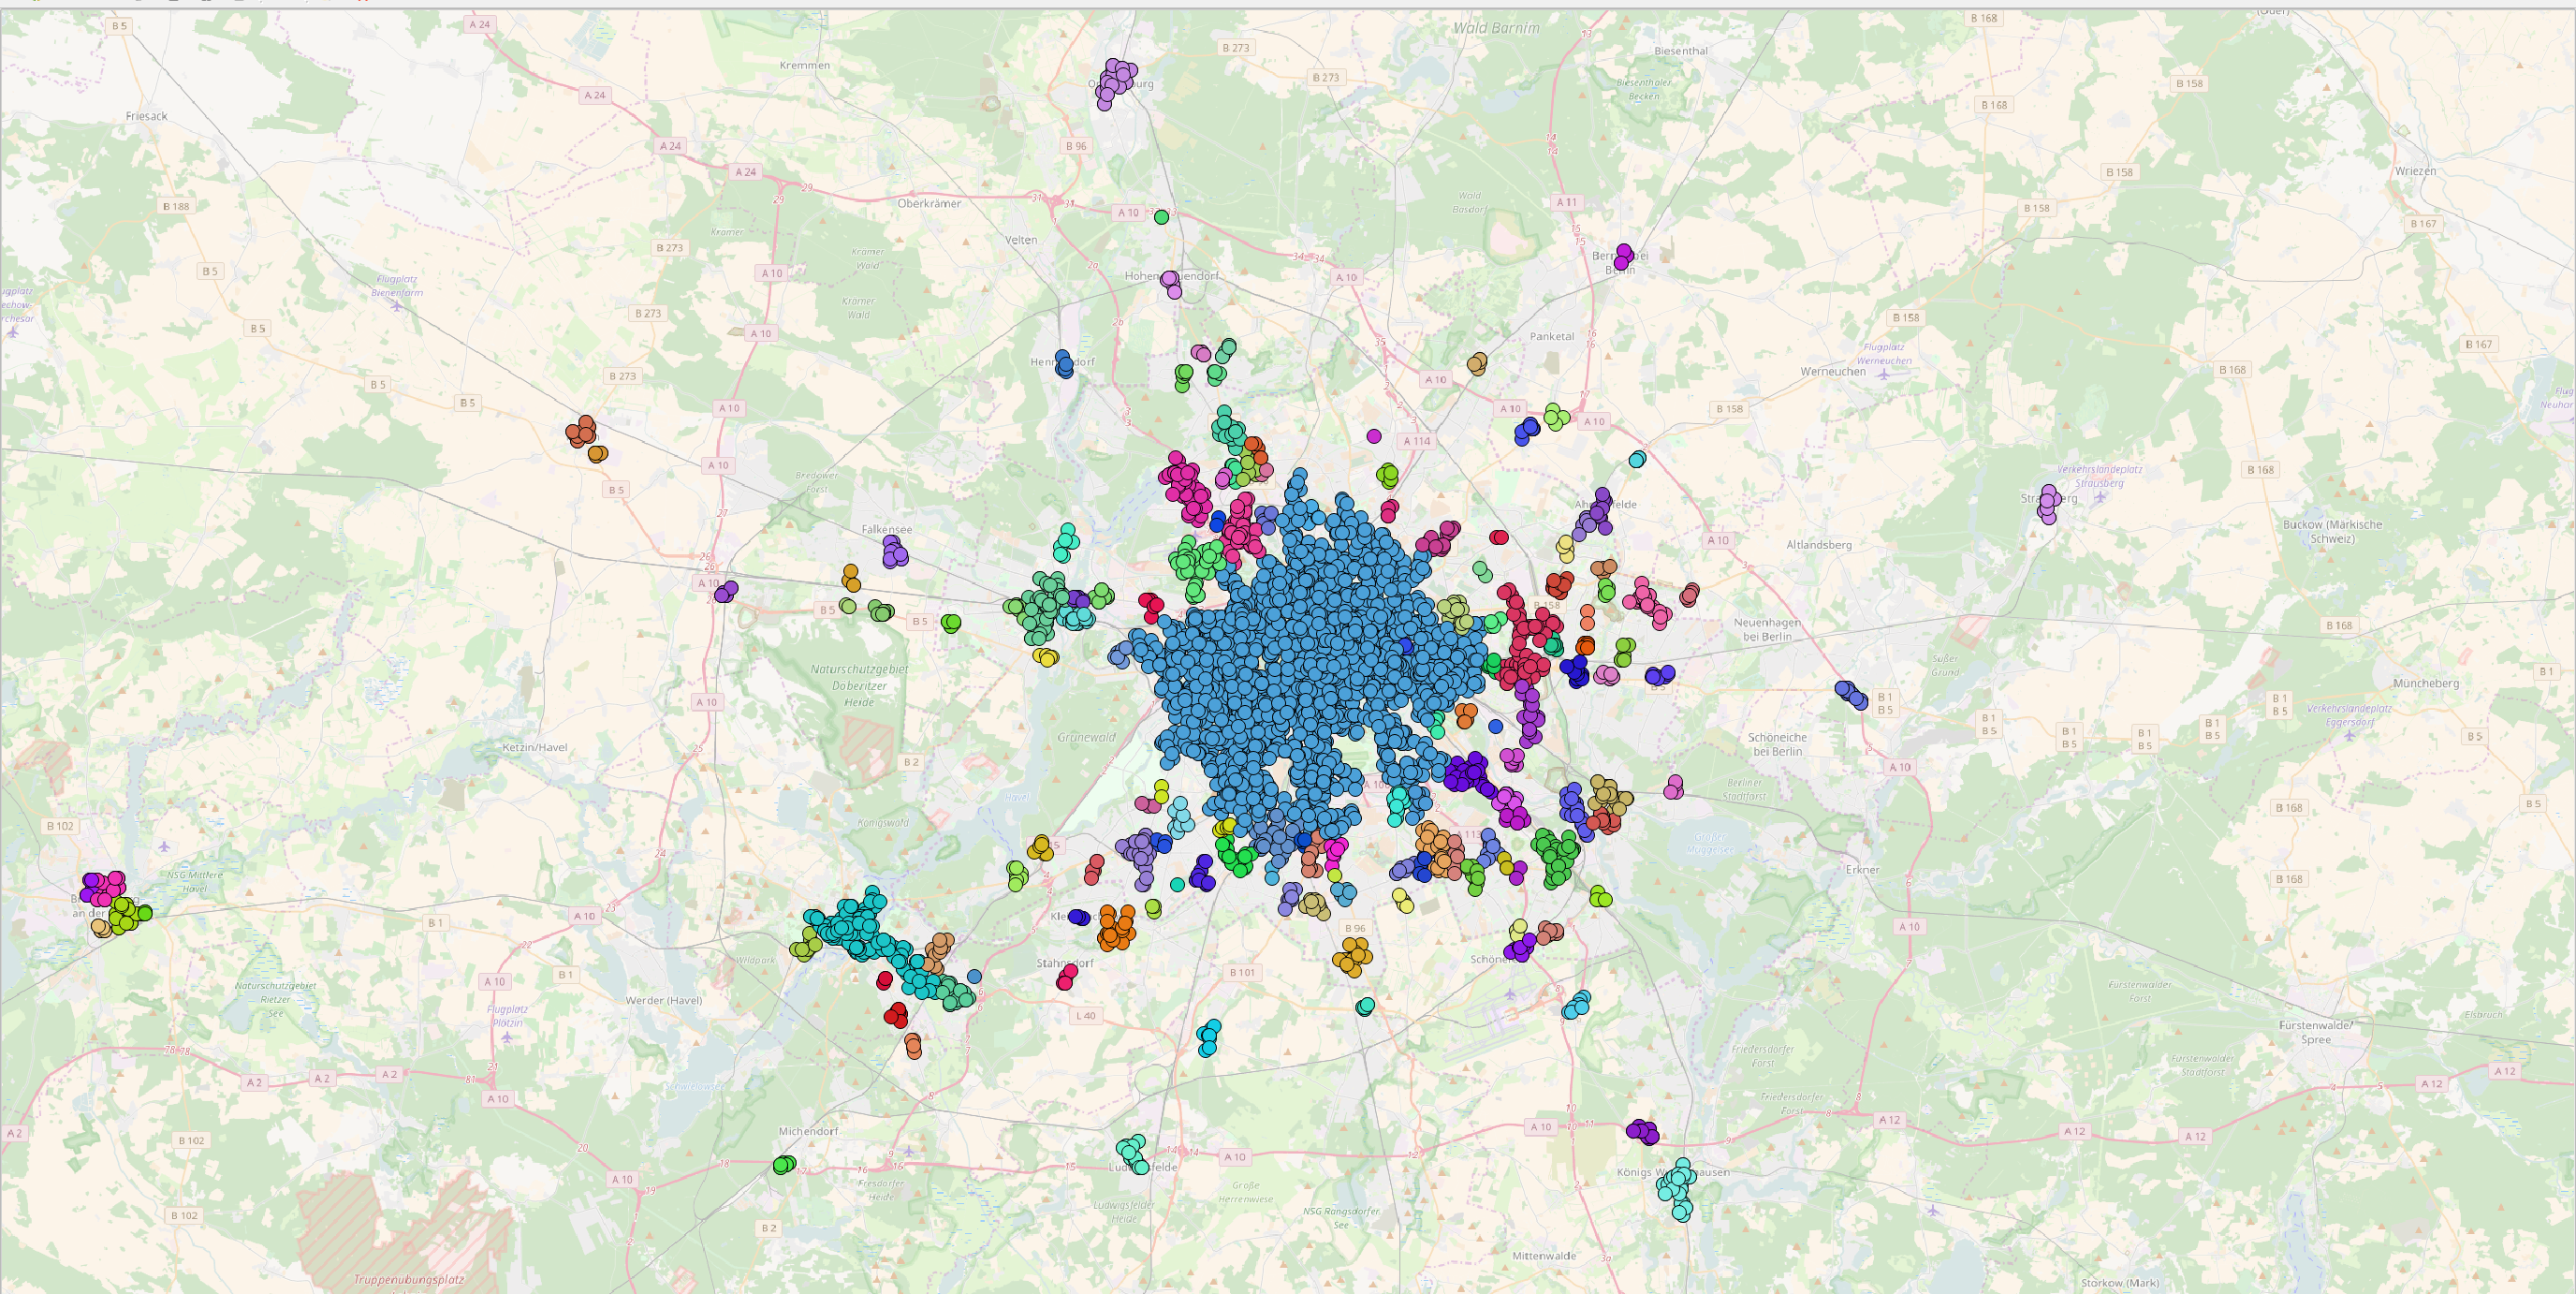
\includegraphics[width=0.8\textwidth]{images/big_cluster.PNG}\\
	\caption{ Huge cluster problem in central Berlin problem when trying to detect clusters outside the center. }
	\label{fig:huge_cluster}
\end{figure}
To solve the problem of not detecting clusters in less dense areas we implemented an area version of DBSCAN. This version ran DBSCAN on different areas of varying density with different \textit{eps}. To demonstrate this we divided Berlin and surrounding area into three different boxes of increasing density, as seen in figure \ref{fig:boxes}. Each point was assign to its specific box and a \textit{DBSCAN on Spark} was executed on each box and finally the result was merged. The goal was to capture more clusters in less dense regions. 
\begin{figure}[!ht]
	\centering
	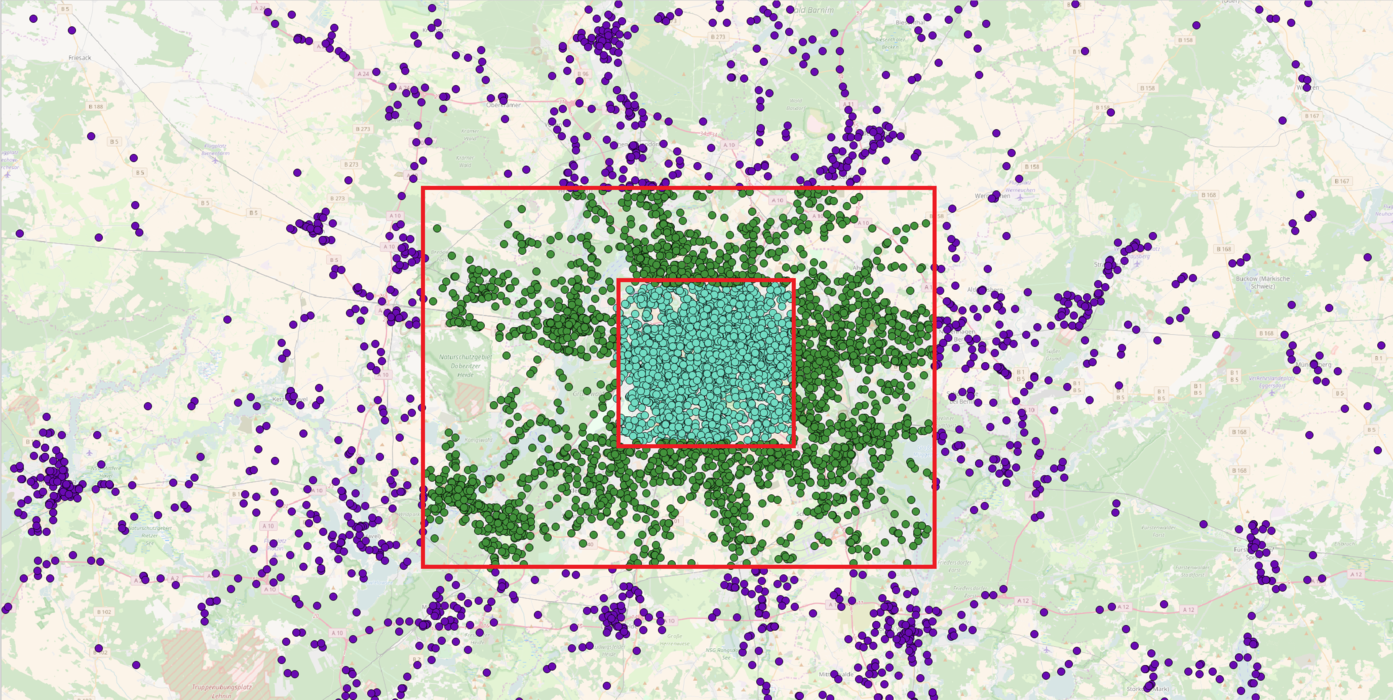
\includegraphics[width=0.8\textwidth]{images/boxes.PNG}\\
	\caption{  Berlin and surrounding area divided into boxes. On each box a separate\textit{ DBSCAN on spark} is ran with different parameters. }
	\label{fig:boxes}
\end{figure}
The \textit{eps} of each outer area was increased from the previous one and the histogram in figure \ref{fig:clusters_versions} proves the feasibility of the area implementation, we capture more clusters outside of inner Berlin with the new area version. The first version runs the original DBSCAN version without using boxes, the second version divides greater Berlin into two boxes, inner and outer Berlin. Finally, the third version uses three boxes; inner, middle and outer Berlin.\begin{figure}
    \centering
    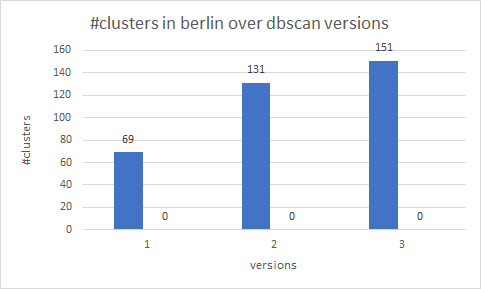
\includegraphics[width=0.5\textwidth]{images/clusters_versions.png}\\
    \caption{ Histogram over found clusters running the different area DBSCAN versions.}
    \label{fig:clusters_versions}
\end{figure}


\begin{figure}
	\centering
	\begin{subfigure}
		\centering
		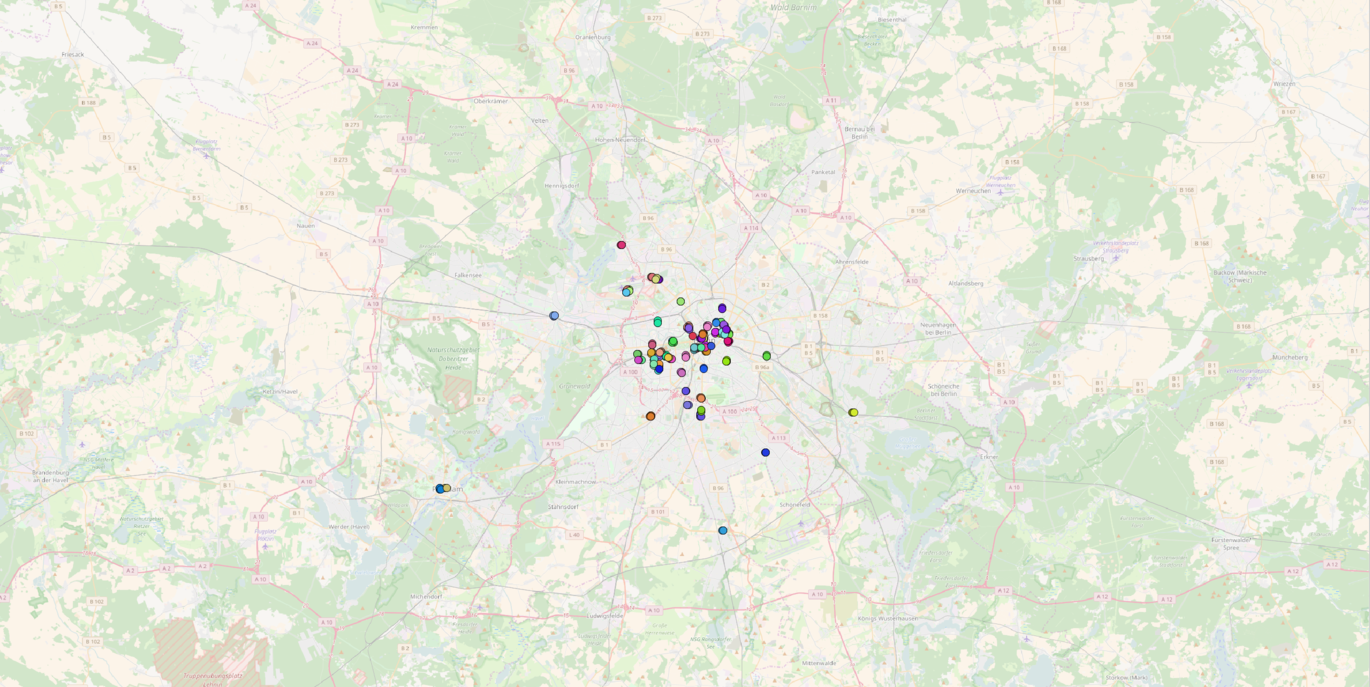
\includegraphics[width=0.8\textwidth]{images/1_v.PNG}\\
        \caption{ Version 1. Result of running original DBSCAN without boxes. \textit{eps} = \textit{minimum distance}  on dataset}
        \label{fig:1_v}
	\end{subfigure}%
	\begin{subfigure}
    \centering
        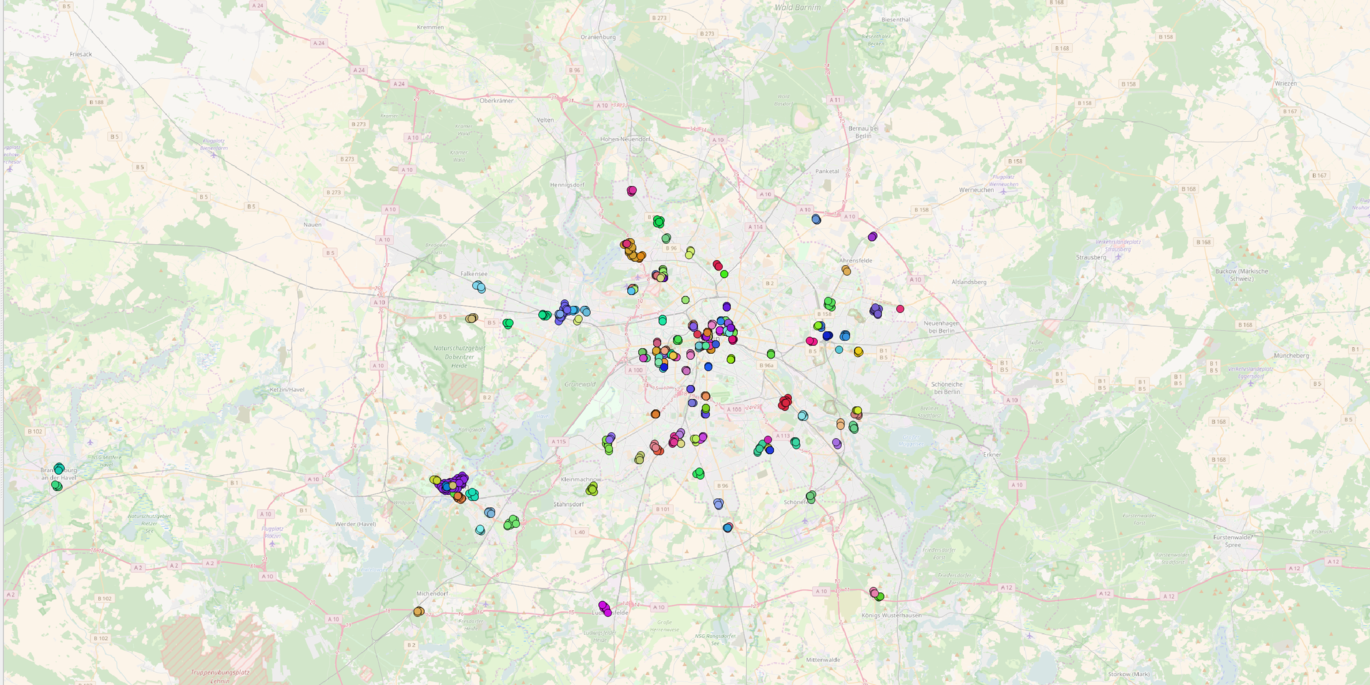
\includegraphics[width=0.8\textwidth]{images/2_v.PNG}\\
        \caption{ Version 2. Result of running DBSCAN with two boxes.        \textit{eps} = \textit{2 * minimum distance}  on dataset}
        \label{fig:2_v}
    \end{subfigure}% 
	\begin{subfigure}
		\centering
	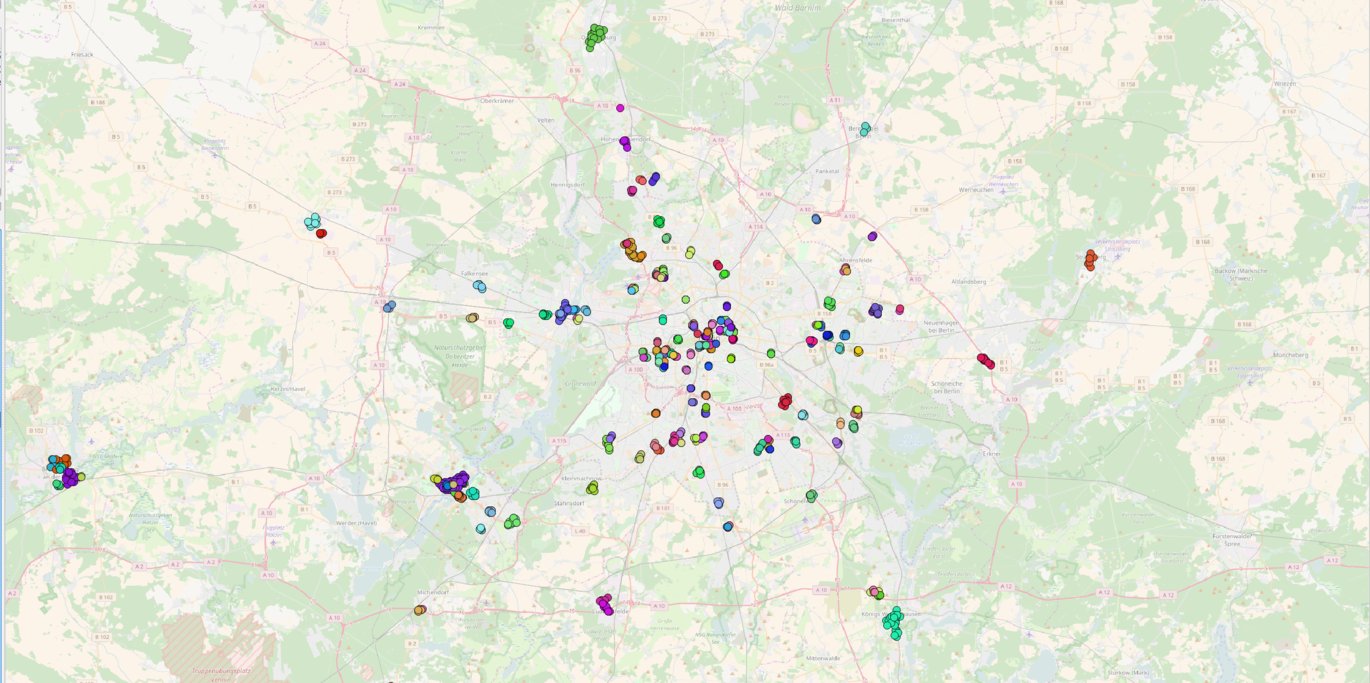
\includegraphics[width=0.8\textwidth]{images/3_v.PNG}\\
        	\caption{ Version 3. Result of running the area extension of DBSCAN with three boxes. Parameter \textit{eps} = \textit{minimum distance}  for inner area, \textit{eps} = 3 * \textit{minimum distance}  for middle area, and  \textit{eps} = 5 * \textit{minimum distance} for outer area. We find much more found clusters than original DBSCAN version}
        	\label{fig:3_v}
	\end{subfigure}
\end{figure}
\FloatBarrier

\section{User movement graph}
This section describes the evaluation of the results obtained from the user movement graph. 

We choose the clusters in and around Berlin for our evaluation and worked with the data from the same. Different properties were extracted from the graph like trip count, indegree and outdegree of the vertices, PageRank and Betweenness centralities. It was our assumption that these values should help us identify areas of interest in the city as well as provide an insight into user movement patterns. We plotted the distribution of values in python to get a better idea of the range and characteristics of the values. Plotting the data also helped us identify suitable thresholds for the properties. These thresholds were needed in order to obtain clusters of importance i.e. vertices with the highest values, as well as to examine validity of the results.

\begin{figure}[!ht]
	\centering
	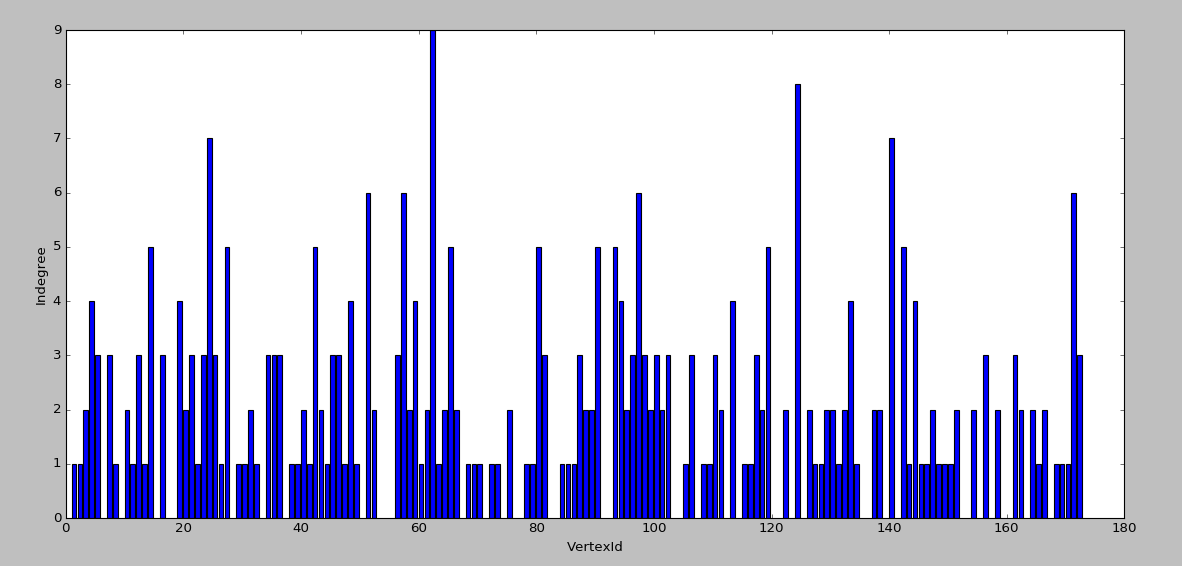
\includegraphics[width=0.7\textwidth]{images/indegree_plot.png}
	\caption{ Plot of indegree values of vertices}
	\label{:Indegree Plot}
\end{figure} 
\begin{figure}[!ht]
	\centering
	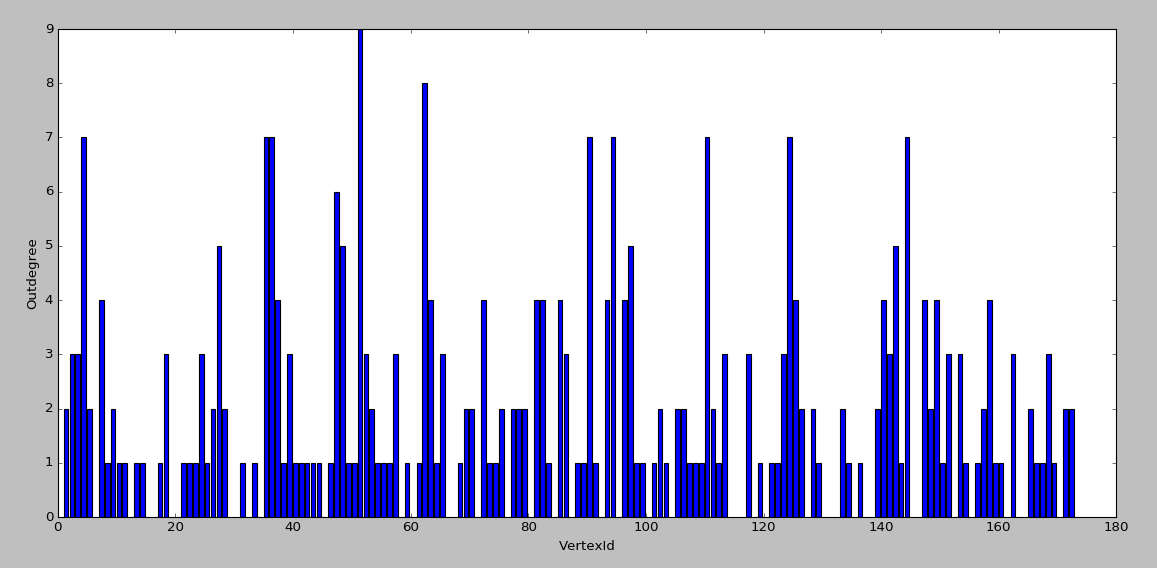
\includegraphics[width=0.7\textwidth]{images/outdegree_plot.png}
	\caption{ Plot of outdegree values of vertices}
	\label{:Outdegree Plot}
\end{figure} 
\begin{figure}[!ht]
	\centering
	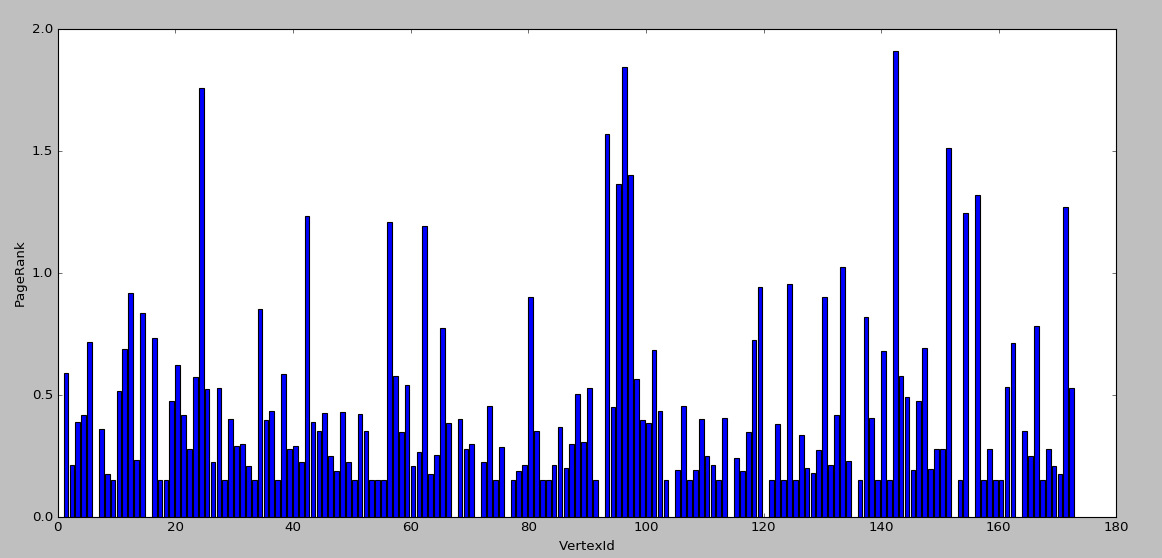
\includegraphics[width=0.7\textwidth]{images/pagerank_plot.png}
	\caption{ Plot of PageRank of the vertices}
	\label{:PageRank Plot}
\end{figure} 
\begin{figure}[!ht]
	\centering
	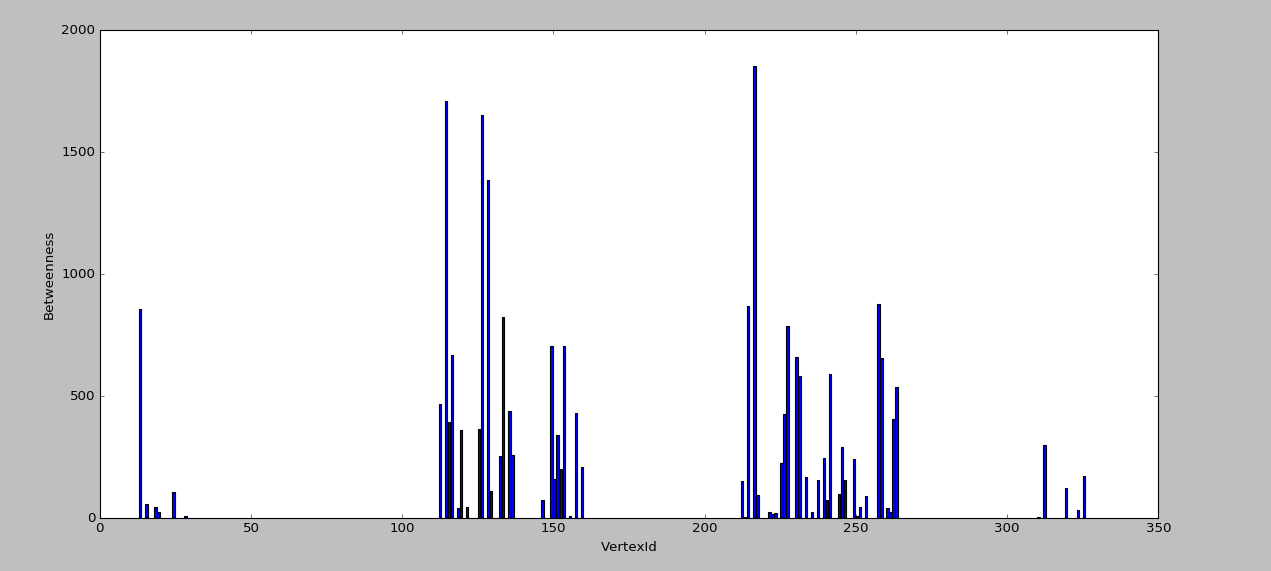
\includegraphics[width=0.7\textwidth]{images/betweenness_plot.png}
	\caption{ Plot of Betweenness of the vertices}
	\label{:Betweenness Plot}
\end{figure}
\FloatBarrier

As seen in the above plots, the values range from 0 ( or default value of 0.15 in case of PageRank) to significantly high values. For example: highest betweenness was 1854.38. Hence we decided to discard the zero values (in case of In,Out degrees and Betweenness) or default values (in case of PageRank) in order to obtain a realistic and meaningful threshold.

\autoref{table:range_threshold}  provides the range and threshold (calculated after discarding the zero or default values) in each case. The mean of the distributions were selected as threshold.  

\begin{table}[ht]
\caption{Range and thresholds}
\centering 
\begin{tabular}{c c c}
\hline
Property & Range & Mean \\[0.5ex]
\hline
Indegree & [0-9] & 2.46 \\
Outdegree & [0-9] & 2.44 \\
PageRank & [0.15 -1.909] & 0.522 \\
Betweenness & [0-1854.38] & 342.33 \\ [1ex]
\hline
\end{tabular}
\label{table:range_threshold}
\end{table}

For each of the properties, vertices with values above the threshold were plotted on the map of Berlin using QGIS. Once the values were mapped to actual physical location in a city, we could understand and evaluate the results. The results are presented in the images from \autoref{:Indegree QGIS}  to \autoref{:Betweenness QGIS} 
\begin{figure}[!ht]
	\centering
	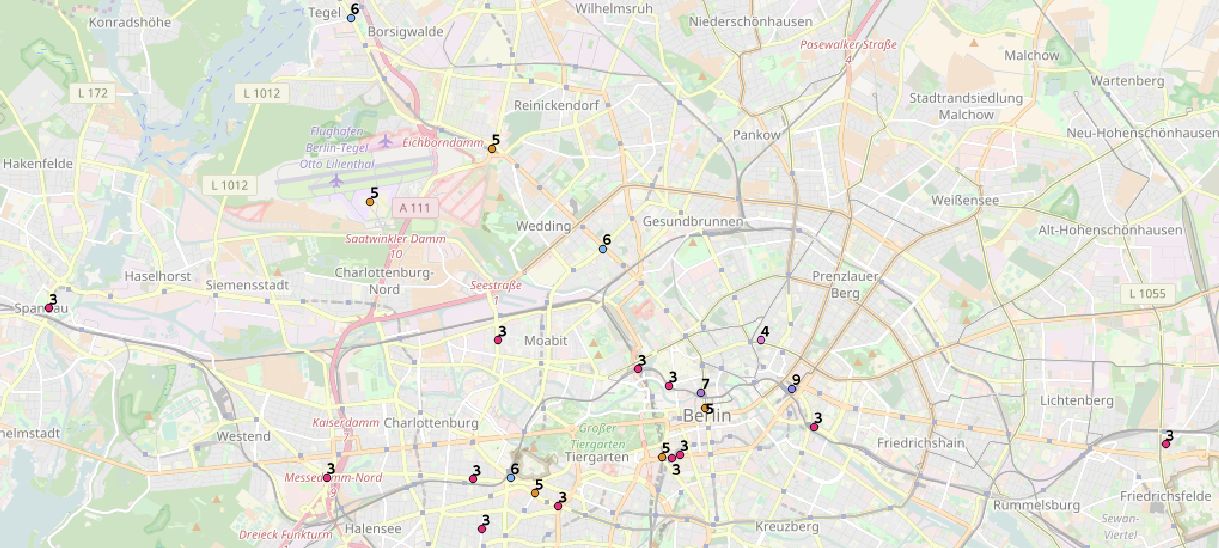
\includegraphics[width=0.7\textwidth]{images/indegree_qgis.png}
	\caption{ Indegree values of places in Berlin}
	\label{:Indegree QGIS}
\end{figure} 
\begin{figure}[!ht]
	\centering
	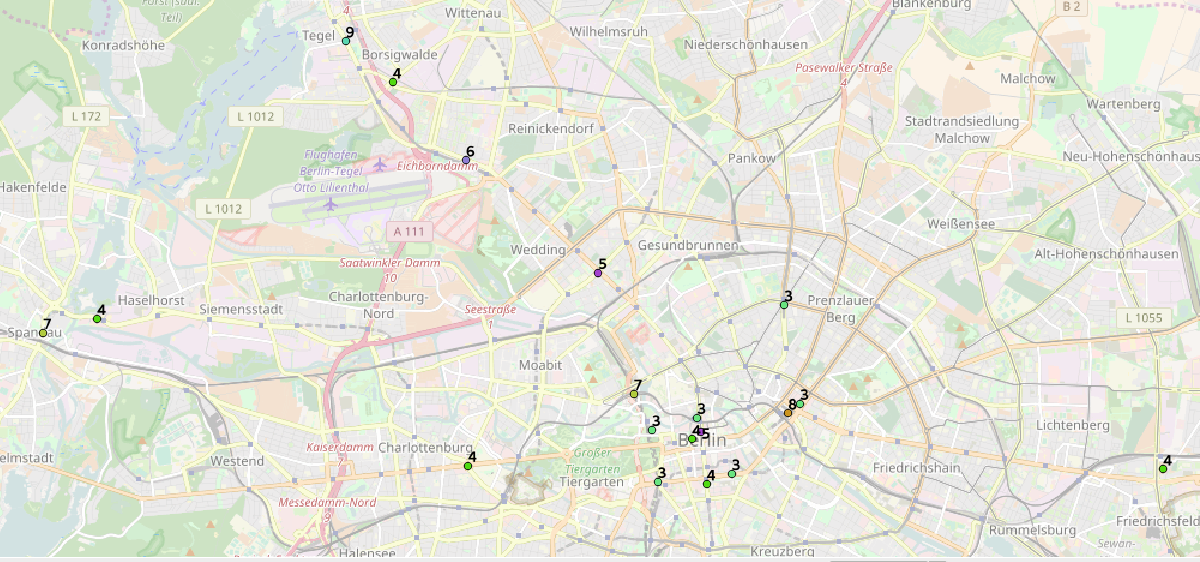
\includegraphics[width=0.7\textwidth]{images/outdegree_qgis.png}
	\caption{ Outdegree values of places in Berlin}
	\label{:Outdegree QGIS}
\end{figure} 
\begin{figure}[!ht]
	\centering
	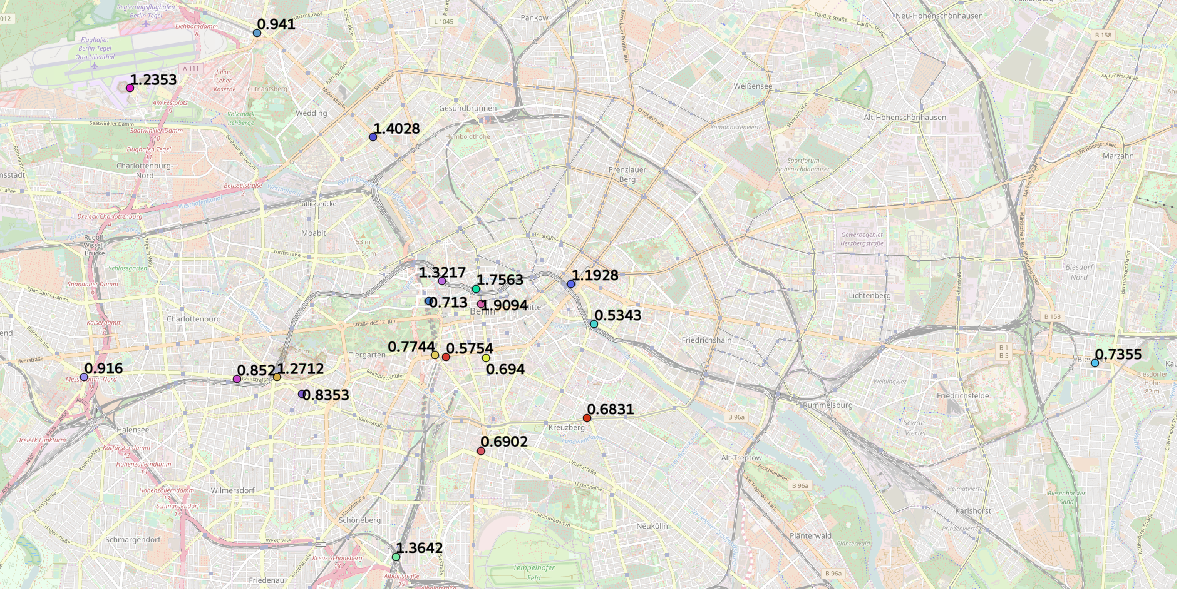
\includegraphics[width=0.7\textwidth]{images/pagerank_qgis.png}
	\caption{PageRank values of places in Berlin}
	\label{:PageRank QGIS}
\end{figure} 
\FloatBarrier

\begin{figure}[!ht]
	\centering
	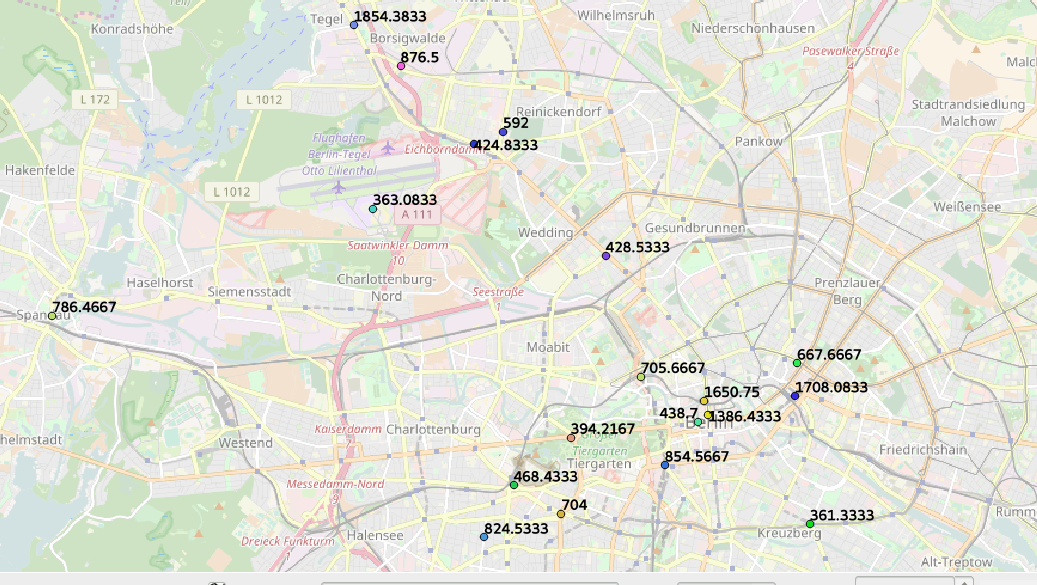
\includegraphics[width=0.7\textwidth]{images/betweenness_qgis.png}
	\caption{ Betweenness values of places in Berlin}
	\label{:Betweenness QGIS}
\end{figure}
\FloatBarrier

From the above images we could identify that the areas of high indegrees and outdegrees were residential areas or areas of special importance in the city like business or shopping destinations or major transport hubs. For example: Alexanderplatz in Berlin has both highest indegree (=9) and second highest outdegree (=8). The values made sense as Alexanderplatz is not only a popular spot for shopping and dining, it is also a major transport hub and is equally popular among locals residents and tourists.

In the following section, we present in-and out-degree values of a few chosen well-known places in Berlin and our explanations for the same.

\begin{table}[ht]
	\caption{Locations and in-\& out-degree values}
	\centering
	\begin{tabular}{c c c}
		\hline
		Index &Place & In-\& Outdegree \\[0.1ex]
		\hline
		1. & Tegel  & 6,9 \\		
		2. & Friedrichstraße & 7,5 \\
		3. & Potsdamer Platz & 5,3 \\			
		4. & Zoologischer Garten & 6,2 \\
		5. & Berlin Hauptbahnhof & 3,7 \\	
		6. & Alexanderplatz & 9,8 \\
		7. & Spandau & 3,7 \\
		8. & Potsdam & 8,7 \\ [1ex]				
		\hline
	\end{tabular}
	\label{table:inout_zones_reasons}
\end{table}

As per our analysis, the locations presented in \autoref{table:inout_zones_reasons} are important locations in Berlin for several reasons such as: transportation hub (Indexes 2,4,5,6,7), popular tourist areas(Indexes 2,3,4,5,6,7), popular shopping and dining areas(Indexes 2,3), proximity to airport(Index 1) or university( Indexes 2,4) and residential areas(Indexes 1,6,7).

Our next target was to learn about movement patterns and connectivity in the city. To achieve this we analyzed the locations with high pagerank and betweenness centralities (refer to \autoref{:PageRank QGIS} and \autoref{:Betweenness QGIS}). A list of locations chosen for our study is presented in \autoref{table:pagerank} and \autoref{table:betweenness}

\begin{table}[ht]
	\caption{Locations with PageRank values}
	\centering
	\begin{tabular}{c c c}
		\hline
		Index &Place & Betweenness\\[0.1ex]
		\hline
		1. & Tegel Airport  & 1.2353 \\		
		2. & S + U Friedrichstraße & 1.7563 \\
		3. & Friedrichstraße & 1.9094 \\		
		4. & Berlin Südkreuz & 1.3642 \\			
		5. & Zoologischer Garten & 1.2712 \\		
		6. & Alexanderplatz & 1.1928 \\				
		7. & Messedamm Nord & 0.916 \\
		8. & Leopoldplatz & 1.4028 \\		
		9. & Potsdam & 0.9556 \\  [1ex]
		\hline
	\end{tabular}
	\label{table:pagerank}
\end{table}

\begin{table}[ht]
	\caption{Locations with betweenness values}
	\centering
	\begin{tabular}{c c c}
		\hline
		Index &Place & Betweenness\\[0.1ex]
		\hline
		1. & Tegel  & 1854.383 \\		
		2. & S + U Friedrichstraße & 1650.75 \\
		3. & Friedrichstraße & 1386.43 \\		
		4. & Potsdamer Platz & 854.567 \\			
		5. & Zoologischer Garten & 468.43 \\		
		6. & Alexanderplatz & 1.1928 \\				
		7. & Spandau & 786.467 \\		
		8. & Potsdam & 869.05 \\  [1ex]
		\hline
	\end{tabular}
	\label{table:betweenness}
\end{table}
\FloatBarrier

We compared the locations in the \autoref{table:inout_zones_reasons} and \autoref{table:pagerank} and noticed that some of the locations in these two tables are different. That is, despite moderate to high in- and out-degree values, the PageRank values of some nodes were not significant. We attributed this to the connectivity among the nodes and assumed that locations mentioned in the\autoref{table:pagerank} were important because of they were connected with other significant locations in the city. We found that indeed these locations were important transport hubs apart from being shopping/tourist attractions or residential localities. For example: Messedamm Nord is close to central bus stop of Berlin, Berlin Südkreuz is a major train station and both these places have good connectivity with the city and other towns nearby. Thus we the results can be inferred as valid.

Next, we analyzed the locations with high betweenness values with the assumption that this result set should provide us with a list of nodes that enjoy a place of influence in the network due to their relative position with  respect to other nodes. On assessing the results in \autoref{table:betweenness}, we found that our assumptions were true as these nodes are part of many important transport routes and serve as change-over points between different modes of transport. We have already sighted examples of Alexanderplatz and Zoologischer Garten in this respect. Equally important examples were that of the cities of Spandau and Potsdam. From the results we can conclude that we have been able to identify key locations in the city that denote the choice of routes by users.

To further validate the inferences drawn from the centrality values, we checked the strongly connected components of the graph. Not surprisingly the nodes appearing in the above tables featured in those as well. As seen in 
\autoref{:connected_component}, the strongly connected component comprises of the key locations were already identified by us. 
\begin{figure}[!ht]
	\centering
	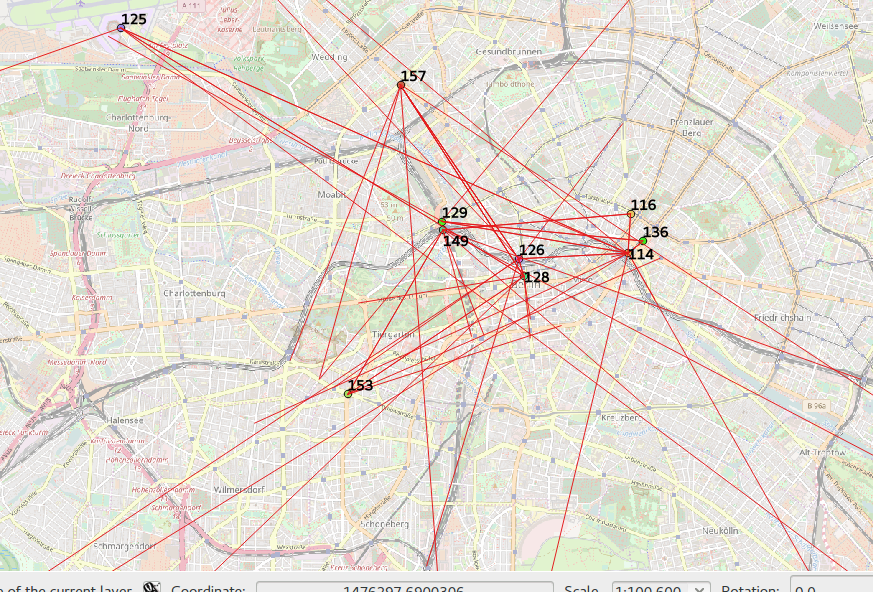
\includegraphics[width=0.7\textwidth]{images/connected_component.png}
	\caption{Largest strongly connected component in Berlin}
	\label{:connected_component}
\end{figure}  
\FloatBarrier

After identifying popular locations and connectivity choices of users, our next focus was to identify key routes in the city. As already described in \autoref{cha:graph1}, trip count values indicate the number of edges between each pair of nodes. We used trip counts of node-pairs to identify the nodes with highest traffic.
\begin{figure}[!ht]
	\centering
	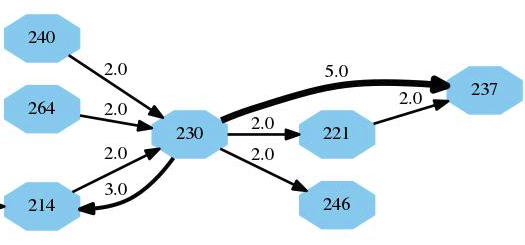
\includegraphics[width=0.5\textwidth]{images/max_tripcount.png}
	\caption{Edges with the maximum trip counts}
	\label{:tripcount}
\end{figure}  
\begin{figure}[!ht]
	\centering
	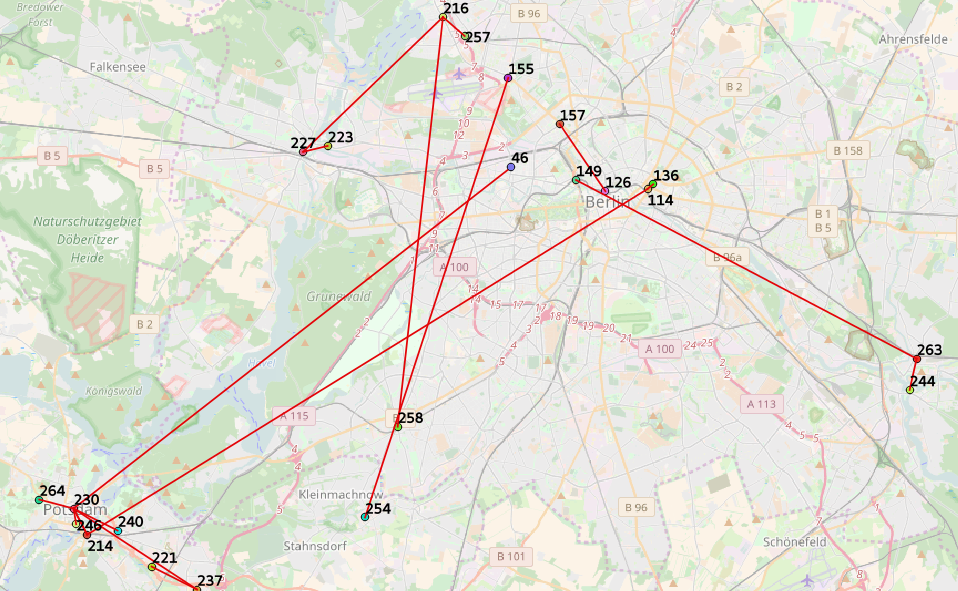
\includegraphics[width=0.7\textwidth]{images/edges_city.png}
	\caption{Popular routes in the city}
	\label{:edgescity}
\end{figure} 
\FloatBarrier

From \autoref{:edgescity} we can observe that the edges with high traffic correspond to routes between key locations in Berlin and neighboring cities. This result matches the results we already obtained from degree and centrality values and confirms our initial assumptions.

Thus we can conclude that by representing user movement data in the form of a graph and using its properties, we could determine key locations, key routes and connectivity of the city. 
  